\documentclass{article}

\usepackage[final, nonatbib]{neurips_2024}

\usepackage[utf8]{inputenc} % allow utf-8 input
\usepackage[T1]{fontenc}    % use 8-bit T1 fonts
%\usepackage{hyperref}       % hyperlinks
%\usepackage{url}            % simple URL typesetting
\usepackage{booktabs}       % professional-quality tables
\usepackage{amsfonts}       % blackboard math symbols
\usepackage{nicefrac}       % compact symbols for 1/2, etc.
\usepackage{microtype}      % microtypography
\usepackage{xcolor}         % colors

\usepackage{url}
\def\UrlBreaks{\do\/\do-}
\usepackage{breakurl}
\usepackage[breaklinks]{hyperref}

\usepackage{amsmath}
\usepackage{graphicx}
\usepackage{threeparttable}
\usepackage{wrapfig}
\usepackage[normalem]{ulem} 
\useunder{\uline}{\ul}{}

\title{Tokenization Revisited: Balancing Efficiency and Linguistic Integrity in Multilingual NLP}

\author{
M. Ali Bayram$^1$, Ali Arda Fincan$^2$, Ahmet Semih Gümüş$^2$, Sercan Karakaş$^3$, Banu Diri$^1$\\
$^1$Yıldız Technical University, $^2$Yeditepe University, $^3$OpenAI \\
\texttt{malibayram20@gmail.com}
}

\begin{document}
\maketitle

\begin{abstract}
  Tokenization is a critical preprocessing step in natural language processing (NLP), shaping how effectively large language models (LLMs) capture linguistic and semantic nuance. This paper presents a comprehensive framework for tokenization standards that prioritize morphological and semantic integrity, especially for morphologically complex and low-resource languages. Using Turkish as a case study, we evaluate eight LLM-derived tokenizers on a subset of the Massive Multitask Language Understanding (MMLU) benchmark. Our analysis goes beyond conventional efficiency metrics—such as vocabulary size, token count, and processing speed—by incorporating linguistic token percentages and semantic purity to assess how faithfully tokenizers preserve linguistic structure. The results highlight that language-specific tokenization strategies substantially improve downstream performance, even when training data is limited, and show that larger model parameters do not inherently yield better tokenization or enhanced results. These findings underscore the need to balance computational efficiency with linguistic alignment, tailoring tokenization methods to the morphological properties of each language. The proposed framework is adaptable to various linguistic contexts, guiding the development of tokenizers that improve model accuracy, robustness, and versatility. Future work will explore advanced morphological analysis, domain-specific customization, and cross-linguistic comparisons to further refine tokenization practices and advance the state of multilingual NLP.
  
  \textbf{Keywords:} Tokenization Standards, Morphological Integrity, Semantic Fidelity, Low-Resource Languages, Multilingual NLP, Morphologically Complex Languages
  \end{abstract}
\section{Introduction}

Tokenization is a critical preprocessing step in natural language processing (NLP) that directly influences the effectiveness and efficiency of language models. This process involves breaking text into smaller units, such as words, subwords, or characters, which serve as the fundamental input for models. While tokenization is a universal requirement across languages, its complexity increases for morphologically rich and agglutinative languages like Turkish, where a single word often consists of a root and multiple morphemes, each carrying distinct grammatical or semantic meaning. In such cases, standard tokenization methods may fail to capture fine-grained linguistic features, leading to reduced performance on downstream tasks.

Recent advancements in subword tokenization techniques, such as Byte Pair Encoding (BPE) and SentencePiece, have demonstrated substantial improvements in representing complex linguistic structures across languages. These methods segment words into smaller subword units, enabling models to handle rare and unseen words more effectively. For example, the \texttt{Aranizer-PBE-86k} tokenizer, developed for Arabic, effectively captures the morphological nuances of the language, offering insights into handling similar challenges for other languages, including Turkish \cite{koubaa_githubcomriotu-labaranizer_2024}. These methods are also highly relevant for languages with simpler morphologies, such as English, as they improve pattern recognition and representation efficiency, especially in data-scarce scenarios.

Two critical metrics for evaluating tokenization quality are \textit{token purity} and \textit{token percentage} for a given language. Token purity measures the proportion of generated tokens that align with meaningful linguistic units, such as roots, valid morphemes, or semantically coherent segments. A high token purity ensures that meaningful parts of words are preserved during tokenization, minimizing fragmentation and allowing models to learn linguistic patterns more effectively. The token percentage of a specific language, such as Turkish token percentage (TR \%), indicates the proportion of tokens that are valid words or linguistic units within that language. This metric ensures that tokenization aligns with the target language's linguistic structure, reducing noise from invalid or non-linguistic tokens.

These metrics are not only critical for morphologically rich languages but are universally important across all languages, including English. High token purity and language-specific token percentages allow language models to learn meaningful patterns more effectively, even with limited training data. By ensuring that the semantic integrity of linguistic units is preserved, models can better generalize and perform on downstream tasks without needing large-scale datasets. This is particularly significant for low-resource languages or specialized domains where training data is scarce.

Despite advancements, achieving a balance between tokenization speed, vocabulary size, and linguistic fidelity remains a challenge. Excessive fragmentation can dilute semantic meaning, while overly coarse tokenization may overlook critical linguistic details. This balance is crucial not only for morphologically rich languages like Turkish but also for improving performance and efficiency in simpler languages \cite{neubeck_so_2024}.

This paper evaluates tokenizers for Turkish using the MMLU benchmark, a widely recognized evaluation suite for language models. By analyzing tokenizers based on token purity, token percentage, vocabulary size, and processing speed, we aim to identify the most effective approaches for Turkish NLP tasks. The insights gained from this study contribute to developing optimized tokenization strategies that can benefit all languages, ultimately advancing the accuracy and efficiency of NLP models across diverse linguistic settings.
\section{Related Work}

Tokenization plays a fundamental role in natural language processing (NLP), directly influencing the performance, efficiency, and accuracy of large language models (LLMs). Recent research has explored various tokenization strategies and their downstream impacts, aiming to balance linguistic fidelity, computational efficiency, and model scalability.

The \textit{Arabic Tokenizers Leaderboard} \cite{rashad_arabic_nodate} benchmarks tokenizers for Arabic, using datasets such as \texttt{rasaif-translations} and \texttt{Moroccan Arabic Wikipedia}, highlighting the unique challenges posed by Arabic's diverse dialects and orthographic complexity. Tools like \textit{AraNizer} \cite{koubaa_githubcomriotu-labaranizer_2024} leverage subword-based techniques, such as Byte Pair Encoding (BPE) and SentencePiece, to better capture the morphological nuances of Arabic and enhance downstream performance.

Similarly, the \textit{NbAiLab Tokenizer Benchmark} \cite{rosa_nbailabtokenizer-benchmark_2024} evaluates tokenization strategies for Scandinavian languages, emphasizing the critical need for language-specific adaptations in multilingual contexts. For German, Diewald et al. \cite{diewald_tokenizing_2022} assessed tokenizers like \texttt{KorAP-Tokenizer} and \texttt{SoMaJo}, achieving high accuracy in token boundary detection while ensuring computational efficiency for large-scale corpora.

A significant contribution to multilingual tokenization comes from the EuroLLM team, which emphasizes the importance of designing tokenizers with large vocabularies to support diverse linguistic structures \cite{martins_eurollm_2024}. By employing a Byte Pair Encoding (BPE) tokenizer with byte fallback and a vocabulary of 128,000 pieces, EuroLLM achieves a balance between low fertility (tokens per word) and parameter efficiency. Their findings indicate that vocabulary size is a critical factor in determining a tokenizer’s ability to efficiently process multiple languages, including European and non-European ones. EuroLLM's comparison of fertility metrics across tokenizers, such as those from Mistral, LLaMA-3, and Gemma, further underscores the trade-offs between large vocabularies and computational cost.

Efficiency advancements have also been demonstrated in GitHub's faster BPE implementation \cite{neubeck_so_2024}, which significantly improves scalability for tasks requiring billions of tokens. This aligns with EuroLLM’s approach of optimizing tokenization to enhance downstream task performance while maintaining computational efficiency.

Rust et al. \cite{rust_how_2021} highlight the effectiveness of monolingual tokenizers tailored to specific languages, showing notable downstream improvements for morphologically rich languages. Similarly, Lin et al. \cite{lin_not_nodate} propose Selective Language Modeling (SLM), which assigns utility scores to tokens and selectively trains on high-utility tokens, reducing noise and enhancing training efficiency. This approach is particularly relevant for languages like Turkish, where preserving meaningful tokens is essential for capturing linguistic richness.

The studies discussed collectively emphasize the necessity of tokenization strategies that balance linguistic integrity, computational efficiency, and downstream performance. Building on these advancements, this study evaluates tokenizers for Turkish, employing metrics such as token purity, vocabulary size, and processing speed. By integrating insights from multilingual projects like EuroLLM and tailoring techniques for morphologically rich languages, this work advances the understanding and optimization of tokenization for diverse linguistic contexts.
\section{Methodology}

This study focuses on evaluating tokenization strategies for morphologically rich and agglutinative languages, using Turkish as a representative example. While the primary emphasis is on Turkish, the methodology is designed to be flexible and applicable to other languages that present similar challenges in tokenization.

To conduct this evaluation, we utilize the Turkish MMLU dataset \cite{bayram_turkish_nodate}, which contains 6,200 multiple-choice questions covering a diverse range of subjects. This dataset is prepared by extracting questions and answers from a preprocessed resource stored in a Hugging Face repository \cite{bayram_turkish_nodate}. The resulting text corpus, consisting of numerous sentences combined into a single dataset, ensures broad coverage of various linguistic structures encountered in Turkish. Although developed using Turkish data, the same framework can be adapted to other languages by applying analogous linguistic tools and resources.

We employ several metrics to assess both the computational and linguistic aspects of tokenization:

\textbf{Vocabulary Size:}  
The total number of unique tokens (e.g., words, subwords, characters) that a tokenizer can produce. For example, a tokenizer with a vocabulary size of 50,000 might include tokens such as \texttt{"cat"} or \texttt{"run"}, as well as subword units like \texttt{"run"} and \texttt{"ning"} to handle words like \texttt{"running"}. Larger vocabularies can capture more nuanced linguistic patterns, but excessively large vocabularies may increase complexity and memory usage, while smaller vocabularies may fail to represent rare words adequately.

\textbf{Total Token Count:}  
The total number of tokens generated after applying the tokenizer to the entire dataset. For instance, the sentence \texttt{"I love programming languages"} might be split into [\texttt{"I"}, \texttt{"love"}, \texttt{"programming"}, \texttt{"languages"}] using a space-based tokenizer, resulting in four tokens. A subword-based tokenizer might generate [\texttt{"I"}, \texttt{"love"}, \texttt{"program"}, \texttt{"ming"}, \texttt{"languages"}], producing five tokens. Lower total token counts generally imply more compact representations, potentially improving efficiency.

\textbf{Processing Time:}  
The time (in seconds) required to tokenize the entire dataset, reflecting computational efficiency. For example, if a corpus of one million words is processed in 3.2 seconds, the processing time is 3.2 seconds. Faster tokenization is advantageous for large-scale training and real-time applications.

\textbf{Token Percentage (\%TR):}  
A linguistic metric that measures how many tokens correspond to valid words or morphemes in the target language. Consider the sentence \texttt{"Cats are playing"} tokenized as [\texttt{"Ca"}, \texttt{"ts"}, \texttt{"are"}, \texttt{"play"}, \texttt{"ing"}]. If \texttt{"are"}, \texttt{"play"}, and \texttt{"ing"} are considered valid linguistic units, then 3 out of 5 tokens are valid. Thus,  
\[
\%TR = \frac{\text{Valid Tokens (3)}}{\text{Total Tokens (5)}} \times 100 = 60\%.
\]
This ensures that tokenization aligns with the language’s morphology by minimizing invalid segments.

\textbf{Pure Token Percentage (\%Pure):}  
This metric evaluates the proportion of tokens that are inherently meaningful and cannot be further decomposed into smaller meaningful parts. For example, in the sentence \texttt{"The students are learning"}, \texttt{"The"} and \texttt{"are"} are pure tokens, while \texttt{"students"} (\texttt{"student"} + \texttt{"s"}) and \texttt{"learning"} (\texttt{"learn"} + \texttt{"ing"}) are not pure because they can be split into smaller units. If a tokenizer produces 100 unique tokens and 70 of them are pure, we have:  
\[
\%Pure = \frac{\text{Pure Tokens (70)}}{\text{Unique Tokens (100)}} \times 100 = 70\%.
\]

To ensure accurate morphological analysis and token validation, we rely on language-specific tools such as the ITU Turkish NLP Web Service \cite{eryigit_itu_2014} and the Kalbur library \cite{aksoy_ahmetaxkalbur_2024}. Similar linguistic analyzers and rule-based systems can be integrated for other languages. Computational metrics like processing time and token counts are computed using Python scripts and the Hugging Face Tokenizers library \cite{neubeck_so_2024}, ensuring scalability and adaptability.

All experimental procedures, datasets, and configurations are documented for reproducibility. Although Turkish serves as the primary benchmark in this study, the methodology is transferable to other languages and datasets, offering a generalized approach to evaluating tokenization strategies in diverse linguistic environments.
\section{Results and Analysis}

This study assessed eight tokenizers on a Turkish MMLU dataset of 1,605,376 characters and 198,193 words \cite{bayram_turkish_nodate}. To capture both linguistic fidelity and computational effectiveness, we measured Turkish Token Percentage (TR \%) and Pure Token Percentage (Pure \%), along with processing time, parameter size, and MMLU scores. Incorporating model size into the analysis provides a nuanced view of the trade-offs involved in designing tokenizers for morphologically rich languages.

\begin{table}[h]
\centering
\caption{Tokenizer Benchmark Results}
\label{tab:tokenizer-benchmark}
\resizebox{\textwidth}{!}{
\begin{tabular}{|l|c|c|c|c|c|c|c|c|}
\hline
\textbf{Metric} & \textbf{gemma-2} & \textbf{llama-3.1} & \textbf{EuroLLM} & \textbf{Qwen2.5} & \textbf{aya-exp} & \textbf{Mistral} & \textbf{Phi3.5} & \textbf{gpt4o} \\ \hline
Model Params (B) & 27.2 & 70.6 & 9.2 & 7.6 & 32.3 & 12.2 & 3.8 & Unknown \\ \hline
MMLU Score (\%) & 72.10 & 70.42 & 51.29 & 61.68 & 70.66 & 46.89 & 29.37 & 84.84 \\ \hline
Vocab Size & 256,000 & 128,256 & 128,000 & 151,665 & 255,029 & 131,072 & 32,011 & 200,019 \\ \hline
Token Count & 497,015 & 488,535 & 497,173 & 561,866 & 434,526 & 534,930 & 803,971 & 491,137 \\ \hline
Time (s) & 2.95 & 3.12 & 3.20 & 3.31 & 2.77 & 3.14 & 4.55 & 0.51 \\ \hline
Unique Tokens & 6,383 & 6,823 & 5,226 & 5,752 & 8,562 & 4,354 & 3,640 & 7,615 \\ \hline
Turkish Tokens & 3,104 & 3,125 & 2,457 & 2,320 & 4,338 & 1,971 & 1,599 & 3,209 \\ \hline
TR \% & 48.63 & 45.80 & 47.01 & 40.33 & 50.67 & 45.27 & 43.93 & 42.14 \\ \hline
Pure Tokens & 2,365 & 2,109 & 1,838 & 1,734 & 2,822 & 1,571 & 1,253 & 2,184 \\ \hline
Pure \% & 37.05 & 30.91 & 35.17 & 30.15 & 32.96 & 36.08 & 34.42 & 28.68 \\ \hline
\end{tabular}
}
\end{table}

Table~\ref{tab:tokenizer-benchmark} summarizes these metrics, illustrating how vocabulary size, token counts, runtime, and language-specific alignment interact with downstream performance. Notably, larger parameter sizes do not guarantee superior results. For instance, \texttt{gemma-2} (27.2B parameters) outperformed the considerably larger \texttt{llama-3.1} (70.6B parameters) in Turkish MMLU accuracy, indicating that \texttt{gemma-2}’s tokenizer is better tuned to Turkish morphology. This contrasts with their English MMLU standings, where \texttt{llama-3.1} excels \cite{ai_llama_nodate}, underscoring the language-dependence of tokenizer effectiveness.

\texttt{gemma-2} achieved higher TR \% (48.63\%) and Pure \% (37.05\%) than \texttt{llama-3.1} (45.80\% TR, 30.91\% Pure), emphasizing the importance of language-specific tokenization in capturing morphological structure. Although \texttt{aya-expanse} (32.3B) recorded the highest TR \% (50.67\%), its MMLU score (70.66\%) leaves room for improvement, demonstrating that while linguistic alignment is crucial, it must be balanced with computational efficiency and task optimization.

At the other end of the spectrum, \texttt{o200k-gpt40} achieved the highest MMLU score (84.84\%) and fastest processing time (0.51s), but with a relatively modest TR \% (42.14\%). This trade-off reflects the impact of optimization techniques like distillation and pruning \cite{lacy_gpt-4o_2024,shakrapani_gpt_nodate}, which boost performance and speed at the expense of linguistic fidelity. Similarly, smaller models such as \texttt{Mistral} (12.2B) and \texttt{Phi3.5} (3.8B) struggled on both fronts, demonstrating that limited parameter counts often require more sophisticated tokenization strategies to handle complex morphologies effectively.


Figure~\ref{fig:model_comparison} provides a multidimensional visualization of these trade-offs, plotting MMLU scores against TR \%, with marker size representing parameter count and color encoding Pure \%. This allows for a holistic comparison: models that achieve high TR \% and Pure \% tend to better capture the language’s morphological richness, while those with large parameter counts or specific optimizations may excel in overall performance yet fail to preserve linguistic integrity.

\begin{figure}[h!]
    \centering
    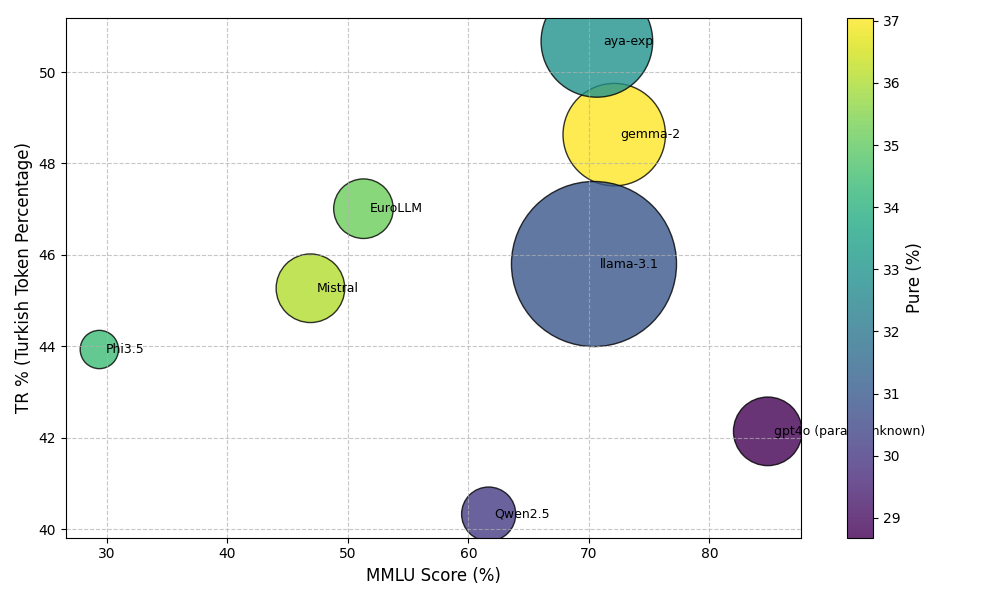
\includegraphics[width=1\textwidth]{model_comparison.png}
    \caption{
    Model Comparison: MMLU vs TR\%, Parameter Size (Unknown for gpt4o), and Pure\%
    }
    \label{fig:model_comparison}
\end{figure}

In summary, these results confirm that linguistic alignment significantly shapes downstream success in morphologically complex settings. Tailored tokenization can help smaller models compete effectively, while even large or optimized models may fall short if their tokenizers are not linguistically attuned.

\section{Yöntem}

Bu çalışma, morfolojik olarak zengin ve eklemeli dillere yönelik tokenizasyon stratejilerini değerlendirmeyi hedeflemekte olup, Türkçe bu bağlamda temsilci bir örnek olarak kullanılmaktadır. Ana odak Türkçe olsa da, yöntem diğer dillerdeki benzer tokenizasyon zorluklarına uyarlanabilir bir esneklikle tasarlanmıştır.

Bu değerlendirmeyi gerçekleştirmek için, çeşitli konuları kapsayan 6.200 çoktan seçmeli sorudan oluşan Türkçe MMLU veri seti kullanılmıştır \cite{bayram_turkish_nodate}. Bu veri seti, Hugging Face deposunda saklanan ön işlenmiş bir kaynaktan soruların ve cevapların çıkarılmasıyla hazırlanmıştır \cite{bayram_turkish_nodate}. Ortaya çıkan metin korpusu, Türkçe'de karşılaşılan çeşitli dilbilimsel yapıları geniş bir kapsama alanıyla içeren birleşik bir veri setine dönüştürülmüştür. Türkçe verileri kullanılarak geliştirilen bu çerçeve, benzer dil araçları ve kaynaklarının uygulanmasıyla diğer dillere de uyarlanabilir.

Bu çalışma kapsamında, tokenizasyonun hem hesaplama hem de dilbilimsel yönlerini değerlendirmek için çeşitli metrikler kullanılmıştır:

\textbf{Sözlük Boyutu:}  
Bir tokenizatörün üretebileceği benzersiz tokenların (ör. kelimeler, alt kelimeler, karakterler) toplam sayısını ifade eder. Örneğin, 50.000 sözlük boyutuna sahip bir tokenizatör \texttt{"cat"} veya \texttt{"run"} gibi tokenları, ayrıca \texttt{"run"} ve \texttt{"ning"} gibi alt kelime birimlerini içerebilir. Daha büyük sözlükler daha karmaşık dilbilimsel yapıları yakalayabilir, ancak aşırı büyük sözlükler karmaşıklığı ve bellek kullanımını artırabilirken, daha küçük sözlükler nadir kelimeleri yeterince temsil edemeyebilir.

\textbf{Toplam Token Sayısı:}  
Tokenizatör uygulandıktan sonra veri setinde üretilen toplam token sayısını ifade eder. Örneğin, \texttt{"I love programming languages"} cümlesi, boşluk tabanlı bir tokenizatörle [\texttt{"I"}, \texttt{"love"}, \texttt{"programming"}, \texttt{"languages"}] olarak ayrıştırıldığında dört token oluşur. Alt kelime tabanlı bir tokenizatör, [\texttt{"I"}, \texttt{"love"}, \texttt{"program"}, \texttt{"ming"}, \texttt{"languages"}] şeklinde beş token üretebilir. Daha düşük toplam token sayıları, daha kompakt temsiller anlamına gelebilir ve bu da verimliliği artırabilir.

\textbf{İşleme Süresi:}  
Veri setinin tamamını tokenize etmek için gereken süreyi (saniye cinsinden) ifade eder ve hesaplama verimliliğini yansıtır. Örneğin, bir milyon kelimelik bir korpus 3.2 saniyede işlenirse, işleme süresi 3.2 saniye olarak kaydedilir. Daha hızlı tokenizasyon, büyük ölçekli eğitimler ve gerçek zamanlı uygulamalar için avantajlıdır.

\textbf{Token Yüzdesi (\%TR):}  
Hedef dilde geçerli kelimelere veya morfemlere karşılık gelen tokenların oranını ölçen bir dilbilimsel metriktir. Örneğin, \texttt{"Cats are playing"} cümlesi [\texttt{"Ca"}, \texttt{"ts"}, \texttt{"are"}, \texttt{"play"}, \texttt{"ing"}] olarak tokenize edilirse, \texttt{"are"}, \texttt{"play"} ve \texttt{"ing"} geçerli dilbilimsel birimler olarak kabul edilir. Bu durumda:  
\[
\%TR = \frac{\text{Geçerli Tokenlar (3)}}{\text{Toplam Tokenlar (5)}} \times 100 = 60\%.
\]
Bu metrik, tokenizasyonun dilin morfolojisine uygunluğunu sağlar ve geçersiz segmentleri en aza indirir.

\textbf{Saf Token Yüzdesi (\%Pure):}  
Tokenların doğrudan anlamlı olup olmadığını ve daha küçük anlamlı parçalara ayrılıp ayrılamayacağını değerlendiren bir metriktir. Örneğin, \texttt{"The students are learning"} cümlesinde, \texttt{"The"} ve \texttt{"are"} saf tokenlardır, ancak \texttt{"students"} (\texttt{"student"} + \texttt{"s"}) ve \texttt{"learning"} (\texttt{"learn"} + \texttt{"ing"}) saf değildir, çünkü daha küçük birimlere ayrılabilirler. Eğer bir tokenizatör 100 benzersiz token üretmiş ve bunların 70’i saf token ise:  
\[
\%Pure = \frac{\text{Saf Tokenlar (70)}}{\text{Benzersiz Tokenlar (100)}} \times 100 = 70\%.
\]

Doğru morfolojik analiz ve token doğrulaması sağlamak için ITU Turkish NLP Web Service \cite{eryigit_itu_2014} ve Kalbur kütüphanesi \cite{aksoy_ahmetaxkalbur_2024} gibi dil araçlarından yararlanılmıştır. Diğer diller için benzer dil analiz araçları ve kurallara dayalı sistemler entegre edilebilir. İşleme süresi ve token sayıları gibi hesaplama metrikleri, Python betikleri ve Hugging Face Tokenizers kütüphanesi \cite{neubeck_so_2024} kullanılarak hesaplanmış ve bu, ölçeklenebilirliği ve uyarlanabilirliği sağlamıştır.

Tüm deneysel prosedürler, veri setleri ve yapılandırmalar çoğaltılabilirlik için belgelenmiştir. Bu çalışmada Türkçe birincil referans olarak kullanılmış olsa da, önerilen yöntem diğer dillere ve veri setlerine uygulanabilir bir yapı sunarak, farklı dilsel bağlamlarda tokenizasyon stratejilerini değerlendirmeye yönelik genel bir yaklaşım sunmaktadır.
\section{Conclusion}

This study introduced a comprehensive framework for evaluating tokenization strategies, emphasizing the importance of preserving linguistic integrity while maintaining computational efficiency. By focusing on metrics such as token purity, Turkish Token Percentage (TR \%), and processing efficiency, we demonstrated that tokenization strategies significantly impact downstream model performance, particularly in morphologically rich languages like Turkish. Our analysis revealed that parameter size alone is not a definitive predictor of performance. For example, \texttt{gemma-2} (27.2 billion parameters) outperformed the larger \texttt{llama-3.1} (70.6 billion parameters) in Turkish MMLU benchmarks, highlighting the critical role of tokenization alignment with linguistic structure. Conversely, general-purpose models such as \texttt{o200k-gpt4}, while excelling in downstream performance due to extensive optimizations, exhibited lower linguistic fidelity, reflecting the trade-offs inherent in task-specific model optimization. These findings emphasize that tailored tokenization strategies, which balance linguistic preservation and computational demands, are essential for achieving robust NLP performance across diverse languages. The proposed framework is not only applicable to Turkish but also adaptable to other languages and domains, providing a foundation for optimizing tokenization methods to improve multilingual NLP applications and enhance the quality of large language models. Future research will expand this framework to include task-specific evaluations and cross-linguistic comparisons to further refine tokenization strategies for diverse linguistic contexts.

\section{Future Work}

This study highlights the importance of linguistic integrity and computational efficiency in tokenization, presenting a framework to guide the development of tokenizers optimized for morphologically rich and low-resource languages. Although several tokenizers were developed as part of this research, these represent only the initial stages of what is possible. As shown in Table~\ref{tab:future-tokenizers}, these tokenizers—such as \texttt{AhmetSemih/tr\_tokenizer} and \texttt{aliarda/turkish\_tokenizer}—demonstrate promising performance, achieving high Turkish Token Percentages (TR \%) and Pure Token Percentages (Pure \%). However, they currently address only a small portion of the challenges inherent in tokenizing morphologically complex languages like Turkish.

\begin{table}[h]
\centering
\caption{Performance Metrics of Tokenizers at Initial Development Stage}
\label{tab:future-tokenizers}
\resizebox{\textwidth}{!}{
\begin{tabular}{|l|c|c|c|c|c|c|c|c|}
\hline
\textbf{Tokenizer} & \textbf{Vocab Size} & \textbf{Token Count} & \textbf{Time (s)} & \textbf{Unique Tokens} & \textbf{Turkish Tokens} & \textbf{TR \%} & \textbf{Pure Tokens} & \textbf{Pure \%} \\ \hline
\texttt{alibayram/tr\_tokenizer} & 30,158 & 476,556 & 2.42 & 11,531 & 11,342 & 98.36 & 11,055 & 95.87 \\ \hline
\texttt{AhmetSemih/tr\_tokenizer} & 59,572 & 451,883 & 2.48 & 13,370 & 13,253 & 99.12 & 13,357 & 99.90 \\ \hline
\texttt{aliarda/turkish\_tokenizer\_256k} & 256,000 & 488,267 & 2.51 & 13,631 & 13,351 & 97.95 & 12,981 & 95.23 \\ \hline
\texttt{aliarda/turkish\_tokenizer} & 58,526 & 451,936 & 2.34 & 13,268 & 13,170 & 99.26 & 13,256 & 99.91 \\ \hline
\end{tabular}
}
\end{table}

Despite these promising results, much work remains to unlock the full potential of these tokenizers. Future improvements will focus on incorporating advanced morphological analysis steps, which will further enhance their capability to capture the rich grammatical and semantic structures of Turkish. These steps may include integrating more sophisticated linguistic rules, handling rare morphemes, and accounting for contextual variations that impact tokenization in complex languages. Such enhancements will not only improve linguistic fidelity but also expand the scope of the tokenizers for diverse NLP applications.

Additionally, future work will explore iterative refinement processes, such as dynamic token generation based on downstream tasks and domain-specific requirements. For instance, the tokenizers could be fine-tuned for specific domains like medical, legal, or technical texts to ensure high performance in specialized applications. Moreover, incorporating unsupervised and semi-supervised learning approaches into the tokenizer development process will help address gaps in morphological and semantic coverage.

Although still in the early stages of development, these tokenizers provide a strong foundation for further innovation. Their initial performance gives hope that, with targeted improvements, they can evolve into robust, versatile tools for tokenizing morphologically rich languages. By implementing these additional steps and conducting further evaluations across languages and tasks, this research aims to establish a new standard for linguistically informed tokenization, ultimately advancing the quality and efficiency of language models in a wide array of applications.

\bibliographystyle{unsrt}
% \bibliographystyle{plain}
\bibliography{tokenizer}

\end{document}